% ============================================================================
% Glavna.tex -- ulazna tacka seminarskog rada.
% Prati pravila iz PRAVILA_PISANJA_PREMA_TEMPLATEU.md:
%   - bosanska jezicka norma,
%   - struktura razdvojena po fajlovima (\include),
%   - sazetak + abstract, uvod u tri cjeline, poglavlja s kratkim uvodima,
%     zakljucak, popis slika, bibliografija.
% Kompajlirati: pdflatex -> bibtex -> pdflatex -> pdflatex
% ============================================================================
\documentclass[12pt,a4paper,oneside]{report}

\usepackage[utf8]{inputenc}
\usepackage[T1]{fontenc}
% Ako lokalni TeX nema bosanski babel, zamijeniti sa [croatian].
\usepackage[bosnian]{babel}

\usepackage{graphicx}
\usepackage{float}
\usepackage{booktabs}
\usepackage{array}
\usepackage{amsmath,amssymb}
\usepackage{listings}
\usepackage{xcolor}
\usepackage[numbers,sort&compress]{natbib}
\usepackage{tikz}
\usetikzlibrary{positioning,arrows.meta,fit,backgrounds}
\usepackage[hidelinks]{hyperref}

\graphicspath{{Slike/}}

% ---- stil za programski kod / UART ispise -----------------------------------
\definecolor{kodSiva}{RGB}{96,96,96}
\definecolor{kodPozadina}{RGB}{246,246,246}
\lstdefinestyle{plain}{
    basicstyle=\ttfamily\small,
    backgroundcolor=\color{kodPozadina},
    commentstyle=\color{kodSiva},
    breaklines=true,
    frame=single,
    rulecolor=\color{kodSiva!40},
    captionpos=b,
    showstringspaces=false,
    tabsize=2
}
\lstset{style=plain}

% ---- podaci o dokumentu -----------------------------------------------------
\newcommand{\NaslovRada}{Portanje aplikacije TetriSaraj na operativni sistem FreeRTOS na platformi RISC-V (Tang Nano 9K / PicoRV32)}
\newcommand{\ImeAutora}{Delaida Muminovi\'c}
\newcommand{\MjestoGodina}{Zenica, 2026.}

\begin{document}

% ---- Naslovna stranica ------------------------------------------------------
\begin{titlepage}
\begin{center}

\vspace*{3.5cm}

{\large Dokumentacija projekta\par}
\vspace{0.8cm}
{\LARGE \bfseries \NaslovRada \par}

\vfill

{\large Autor: \ImeAutora\par}
\vspace{0.6cm}
{\large \MjestoGodina\par}

\end{center}
\end{titlepage}


% ---- Sazetak, kljucne rijeci, abstract, keywords ---------------------------
\chapter*{Sa\v{z}etak}
\addcontentsline{toc}{chapter}{Sa\v{z}etak}

U radu se razmatra portanje postoje\'ce aplikacije TetriSaraj sa golog
mikrokontrolerskog izvr\v{s}avanja na operativni sistem za rad u realnom vremenu
FreeRTOS, na otvorenoj RISC-V platformi. Ciljna platforma je meki procesor
PicoRV32 sintetizovan na razvojnoj plo\v{c}i Tang Nano 9K. Prikazuje se zna\v{c}aj
operativnih sistema za rad u realnom vremenu u kontekstu ugradbenih sistema sa
ograni\v{c}enim resursima, gdje je potrebno uskladiti vremensku predvidljivost,
zauze\'ce memorije i logi\v{c}kih resursa programabilne logike. Cilj rada je
objasniti postupak prevo\dj{}enja monolitne aplikacije u skup zadataka pod
upravom raspore\dj{}iva\v{c}a, kao i postupak uklapanja takvog sistema zajedno sa
video izlazom u stroge resurse niskobud\v{z}etne plo\v{c}e. Metode kori\v{s}tene
pri izradi rada obuhvataju razvoj i prevo\dj{}enje ugradbenog programa, sintezu
digitalnog sklopa, mjerenje na stvarnom hardveru putem serijske veze i pore\dj{}enje
sa rezultatima dobijenim u simulatoru.

\vspace{0.5cm}
\noindent\textbf{Klju\v{c}ne rije\v{c}i:} FreeRTOS, PicoRV32, RISC-V, sinteza,
Tang Nano 9K, ugradbeni sistemi, zamjena konteksta.

\chapter*{Abstract}
\addcontentsline{toc}{chapter}{Abstract}

This paper considers porting the existing TetriSaraj application from bare-metal
execution to the FreeRTOS real-time operating system on an open RISC-V platform.
The target platform is the PicoRV32 soft processor synthesised on a Tang Nano 9K
development board. The importance of real-time operating systems is presented in
the context of resource-constrained embedded systems, where timing
predictability, memory usage and programmable-logic resource usage must be
balanced. The aim of the paper is to explain the process of converting a
monolithic application into a set of scheduler-managed tasks, as well as the
process of fitting such a system together with video output into the tight
resources of a low-cost board. The methods used in the work include embedded
firmware development and compilation, digital-circuit synthesis, measurement on
real hardware over a serial link, and comparison with results obtained in a
simulator.

\vspace{0.5cm}
\noindent\textbf{Keywords:} context switch, embedded systems, FreeRTOS,
PicoRV32, RISC-V, synthesis, Tang Nano 9K.


\tableofcontents

% ---- Opci uvod (ne numerise se) --------------------------------------------
\chapter*{Uvod}
\addcontentsline{toc}{chapter}{Uvod}

Ugradbeni sistemi danas \v{c}ine najve\'ci dio ra\v{c}unarskih ure\dj{}aja u
svakodnevnoj upotrebi, od ku\'cnih aparata do industrijske opreme. Veliki broj
takvih sistema ima zahtjeve za vremenskom predvidljivo\v{s}\'cu, pa se za
njihovo upravljanje koriste operativni sistemi za rad u realnom vremenu. Jedan
od naj\v{c}e\v{s}\'ce kori\v{s}tenih takvih sistema otvorenog koda je FreeRTOS,
koji je dostupan za veliki broj arhitektura procesora. Istovremeno se sve vi\v{s}e
koristi otvorena skupovna arhitektura RISC-V, koja omogu\'cava izradu vlastitih
procesorskih jezgara bez licencnih ograni\v{c}enja. Spajanje ova dva otvorena
pristupa, operativnog sistema otvorenog koda i otvorene procesorske arhitekture,
postaje zanimljiva i aktuelna tema, posebno na jeftinim razvojnim plo\v{c}ama sa
programabilnom logikom.

Razvojna plo\v{c}a Tang Nano 9K, zasnovana na programabilnom logi\v{c}kom polju
(\foreignlanguage{english}{\emph{Field Programmable Gate Array}}, FPGA), pru\v{z}a
pristupa\v{c}an na\v{c}in da se na njoj sintetizuje meki procesor i izvr\v{s}ava
stvarni program. Meki procesor PicoRV32 jednostavna je RISC-V jezgra pogodna za
takve eksperimente. Me\dj{}utim, resursi ovakvih plo\v{c}a su veoma ograni\v{c}eni,
prije svega blokovska memorija i koli\v{c}ina logi\v{c}kih elemenata, pa
uklapanje slo\v{z}enijih sistema postaje in\v{z}enjerski izazov. Upravo to
\v{c}ini portanje cijele aplikacije zajedno sa operativnim sistemom i video
izlazom netrivijalnim zadatkom.

Ovaj rad nastavlja se na postoje\'cu aplikaciju TetriSaraj, koja je izvorno
pisana kao monolitni program bez operativnog sistema. Postavljaju se sljede\'ca
pitanja na koja rad treba odgovoriti. Da li se aplikacija mo\v{z}e prevesti u
skup zasebnih zadataka pod upravom raspore\dj{}iva\v{c}a operativnog sistema
FreeRTOS i dokazati njen rad na stvarnom hardveru? Da li se takav sistem,
zajedno sa video izlazom preko digitalnog multimedijalnog su\v{c}elja
(\foreignlanguage{english}{\emph{High-Definition Multimedia Interface}}, HDMI),
mo\v{z}e uklopiti u stroge resurse plo\v{c}e Tang Nano 9K? Te kona\v{c}no, kolika
je cijena zamjene konteksta na stvarnom hardveru i kako se ona odnosi prema
ranije dobijenim vrijednostima iz simulatora? Pretpostavlja se da je sve to
mogu\'ce uz pa\v{z}ljivo upravljanje memorijom i resursima.

Rad je organizovan na sljede\'ci na\v{c}in. U prvom poglavlju daje se pregled
srodnih radova i smje\v{s}ta vlastiti rad u kontekst postoje\'ce literature.
Drugo poglavlje opisuje hardversku platformu i prilago\dj{}eni port operativnog
sistema FreeRTOS na meki procesor, te osnovni dokaz njegovog rada. Tre\'ce
poglavlje prikazuje postupak razdvajanja aplikacije na zadatke i dokaz njihovog
rada na hardveru bez video izlaza. \v{C}etvrto poglavlje obja\v{s}njava problem
zauze\'ca resursa pri uklapanju cijele igre sa video izlazom i rje\v{s}enja koja
su to omogu\'cila. Peto poglavlje opisuje mjerenje vremena zamjene konteksta na
hardveru i pore\dj{}enje sa simulatorom. \v{S}esto poglavlje izdvaja mogu\'ce
pravce daljnjeg istra\v{z}ivanja. Na kraju rada dat je zaklju\v{c}ak u kojem su
sistematizirani najva\v{z}niji rezultati i doprinosi rada. Nakon zaklju\v{c}ka
nalazi se popis slika i lista kori\v{s}tenih bibliografskih referenci.

% ============================================================================
\chapter{Srodni radovi}
\label{ch:srodni}
% ============================================================================

U ovom poglavlju daje se pregled dosada\v{s}njih istra\v{z}ivanja koja su bliska
temi rada. Cilj je smjestiti vlastiti rad u \v{s}iri kontekst i jasno pokazati
\v{c}ime se on razlikuje od postoje\'ce literature. Najprije se razmatraju radovi
o mjerenju performansi operativnih sistema za rad u realnom vremenu, zatim radovi
o zamjeni konteksta i prekidima na arhitekturi RISC-V, potom radovi o mekim
procesorima na programabilnoj logici, te na kraju radovi o odnosu simulacije i
stvarnog hardvera. Na osnovu tog pregleda izdvaja se pozicija ovog rada.

\section{Mjerenje performansi operativnih sistema za rad u realnom vremenu}
\label{sec:srodni-rtos}

Mjerenje vremena zamjene konteksta uobi\v{c}ajena je metrika pri pore\dj{}enju
operativnih sistema za rad u realnom vremenu. Pore\dj{}enja sistema FreeRTOS i
Zephyr pokazuju da se ovakve veli\v{c}ine izra\v{z}avaju u broju takta, pri \v{c}emu
se za FreeRTOS navodi red veli\v{c}ine od oko dvije stotine dvadeset tri takta na
jezgrama tipa ARM Cortex-M \citep{ulsolutions2022rtos}. Va\v{z}no je naglasiti da
takve vrijednosti mjere u\v{z}u operaciju zamjene konteksta na cjevovodnom
procesoru, dok mjerenja u ovom radu obuhvataju i dodatni tro\v{s}ak rada sa
mehanizmom sinhronizacije na vi\v{s}eciklusnom mekom procesoru, pa se brojevi ne
mogu direktno pore\dj{}ivati bez te ograde.

\section{Zamjena konteksta i prekidi na arhitekturi RISC-V}
\label{sec:srodni-riscv}

Poseban pravac istra\v{z}ivanja bavi se ubrzanjem zamjene konteksta i obrade
prekida na arhitekturi RISC-V. U radu o pro\v{s}irenju CV32RT predla\v{z}u se
mikroarhitekturna pro\v{s}irenja jezgre radi br\v{z}eg ulaska u prekid i br\v{z}e
zamjene konteksta za mikrokontrolere zasnovane na RISC-V \citep{balas2023cv32rt}.
Sli\v{c}no, postoji istra\v{z}ivanje koje zajedni\v{c}ki istra\v{z}uje
mikroarhitekturu procesora i pro\v{s}irenja samog operativnog sistema FreeRTOS sa
ciljem smanjenja latencije zamjene konteksta \citep{scheck2026coexploration}.
Ovi radovi pokazuju da je smanjenje cijene zamjene konteksta aktuelna tema, ali
se oni uglavnom oslanjaju na izmjene hardvera ili jezgre, dok se ovaj rad bavi
mjerenjem nepromijenjenog sistema na postoje\'coj mekoj jezgri.

\section{Meki procesori RISC-V na programabilnoj logici}
\label{sec:srodni-softcore}

Meki procesori na programabilnoj logici predmet su brojnih evaluacija. Procesor
PicoRV32, kori\v{s}ten i u ovom radu, ocijenjen je kao izrazito \v{s}tedljiv po
pitanju resursa i pogodan za ure\dj{}aje sa ograni\v{c}enim resursima
\citep{jahnke2023picorv32}. Takve evaluacije obi\v{c}no se fokusiraju na
zauze\'ce logi\v{c}kih elemenata i propusnost, dok je rad operativnog sistema na
takvoj jezgri i njegovo uklapanje zajedno sa video izlazom rje\dj{}e obra\dj{}ivano.
Upravo to \v{c}ini doprinos ovog rada, jer se uz mjerenje razmatra i prakti\v{c}no
ograni\v{c}enje blokovske memorije pri sintezi.

\section{Odnos simulacije i stvarnog hardvera}
\label{sec:srodni-qemu}

Emulator QEMU \v{s}iroko se koristi za pokretanje ugradbenog softvera, ali je on
funkcijski ta\v{c}an, \v{s}to zna\v{c}i da vjerno opona\v{s}a pona\v{s}anje
instrukcija, ali ne modeluje mikroarhitekturu takovno ta\v{c}no \citep{qemu}.
Zbog toga se vrijednosti takta dobijene u takvom okru\v{z}enju ne mogu bez ograde
tuma\v{c}iti kao vrijednosti na stvarnom \v{c}ipu. Ova osobina direktno opravdava
opreznost pri pore\dj{}enju rezultata iz simulatora \citep{thesisqemu} sa
rezultatima izmjerenim na hardveru, kako je u\v{c}injeno u poglavlju
\ref{ch:mjerenje}.

\section{Pozicija ovog rada}
\label{sec:srodni-pozicija}

Iz pregleda literature mo\v{z}e se uo\v{c}iti obrazac. Mjerenja performansi
operativnih sistema naj\v{c}e\v{s}\'ce se rade na cjevovodnim mikrokontrolerima
tipa ARM Cortex-M, dok se na arhitekturi RISC-V te\v{z}i\v{s}te stavlja na
hardversko ubrzanje zamjene konteksta. Evaluacije mekih procesora fokusiraju se
na resurse, a rje\dj{}e na rad operativnog sistema. Ovaj rad popunjava prazninu
time \v{s}to mjeri nepromijenjeni FreeRTOS na minimalnoj otvorenoj mekoj RISC-V
jezgri na jeftinoj plo\v{c}i, upore\dj{}uje rezultat sa simulatorom i dokumentuje
prakti\v{c}no ograni\v{c}enje sinteze vezano za blokovsku memoriju. Time se
doprinos rada jasno razlikuje od navedenih istra\v{z}ivanja.

\section{Zaklju\v{c}ak poglavlja}
\label{sec:srodni-zakljucak}

U poglavlju je dat pregled srodnih istra\v{z}ivanja iz \v{c}etiri bliske oblasti
i izdvojena je pozicija ovog rada. Pokazano je da postoje\'ca literatura uglavnom
mjeri operativne sisteme na cjevovodnim jezgrama ili predla\v{z}e hardverska
ubrzanja, dok mjerenje nepromijenjenog sistema na minimalnoj mekoj RISC-V jezgri,
zajedno sa pore\dj{}enjem sa simulatorom, ostaje slabije pokriveno. Time je
opravdan pristup koji se razra\dj{}uje u narednim poglavljima.

% ============================================================================
\chapter{Hardverska platforma i FreeRTOS port}
\label{ch:platforma}
% ============================================================================

U ovom poglavlju opisuje se osnova na kojoj po\v{c}iva cijeli rad. Najprije se
predstavlja razvojna plo\v{c}a i meki procesor na kojem se izvr\v{s}ava program,
zatim prilago\dj{}eni port operativnog sistema FreeRTOS za taj procesor, te
na\v{c}in na koji su organizovani memorija i ulazno-izlazni registri sistema na
\v{c}ipu. Na kraju poglavlja prikazuje se osnovni dokaz da operativni sistem
zaista radi na hardveru, jer bez te potvrde nijedan kasniji rezultat ne bi imao
smisla. Ovo poglavlje predstavlja temelj za razumijevanje kasnijih poglavlja u
kojima se aplikacija razdvaja na zadatke i uklapa u stroge resurse plo\v{c}e.

\section{Tang Nano 9K i meki procesor PicoRV32}
\label{sec:platforma-hardver}

Razvojna plo\v{c}a Tang Nano 9K zasnovana je na programabilnom logi\v{c}kom polju
proizvo\dj{}a\v{c}a Gowin, modela GW1NR-9C. Plo\v{c}a se taktuje vanjskim
oscilatorom od 27 megaherca i raspola\v{z}e ograni\v{c}enim skupom logi\v{c}kih
elemenata i blokovske memorije, \v{s}to je kasnije klju\v{c}no za uklapanje
sistema. Na plo\v{c}i je putem sinteze digitalnog sklopa realizovan meki
procesor PicoRV32, jednostavna jezgra zasnovana na otvorenoj skupovnoj
arhitekturi RISC-V \citep{picorv32}. Procesor je konfigurisan za cjelobrojni
skup instrukcija sa mno\v{z}enjem, \v{s}to se u alatima ozna\v{c}ava kao
\foreignlanguage{english}{\emph{rv32im}}.

PicoRV32 je vi\v{s}eciklusna jezgra, \v{s}to zna\v{c}i da svaka instrukcija
tro\v{s}i vi\v{s}e takta. Takva izvedba je mala i \v{s}tedljiva po pitanju
logike, ali sporija po izvr\v{s}enoj instrukciji u odnosu na cjevovodne procesore.
Ta osobina je va\v{z}na za kasnije tuma\v{c}enje izmjerenih vrijednosti, jer se
broj takta po zamjeni konteksta ne mo\v{z}e direktno tuma\v{c}iti kao broj
izvr\v{s}enih instrukcija.

\section{Prilago\dj{}eni port operativnog sistema FreeRTOS}
\label{sec:platforma-port}

FreeRTOS je operativni sistem za rad u realnom vremenu otvorenog koda, dostupan
za veliki broj arhitektura \citep{freertos}. Za potrebe ovog sistema kori\v{s}ten
je prilago\dj{}eni port jezgre verzije V10.5.1 za PicoRV32. Raspore\dj{}iva\v{c}
periodi\v{c}no dobija takt iz vanjskog broja\v{c}a koji generi\v{s}e prekid na
liniji broj pet, podesen na frekvenciju od sto herca. Promjena zadatka, odnosno
zamjena konteksta, pokre\'ce se programskim prekidom na liniji broj \v{s}est.

Va\v{z}na posebnost ovog porta je obavezna upotreba prevodila\v{c}ke opcije koja
isklju\v{c}uje takozvanu relaksaciju, \foreignlanguage{english}{\emph{-mno-relax}}.
Razlog je taj \v{s}to PicoRV32 u kori\v{s}tenoj konfiguraciji pri ulasku u prekid
mo\v{z}e prepisati registre globalnog i nitnog pokaziva\v{c}a, pa se program ne
smije oslanjati na globalni pokaziva\v{c}. Ova naizgled sitna postavka klju\v{c}na
je za ispravan rad sistema i predstavlja primjer pa\v{z}nje koju zahtijeva rad
na niskom nivou.

\section{Memorijska i adresna organizacija sistema na \v{c}ipu}
\label{sec:platforma-memorija}

Sistem na \v{c}ipu razdvaja prostor programa i prostor podataka. Program se
nalazi u zasebnoj memoriji, takozvanom programskom prozoru, dok se podaci i stog
nalaze u radnoj memoriji veli\v{c}ine \v{s}esnaest kilobajta. Pristup
perifernim jedinicama ostvaruje se preslikavanjem u memoriju
(\foreignlanguage{english}{\emph{Memory-Mapped Input/Output}}, MMIO), gdje svaka
periferija zauzima svoj raspon adresa. Serijska jedinica, brojac, op\v{s}ti
ulazi i izlazi te video jedinica imaju odvojene adresne opsege. Pojednostavljena
slika ove organizacije prikazana je na slici \ref{fig:memorija}.

\begin{figure}[H]
\centering
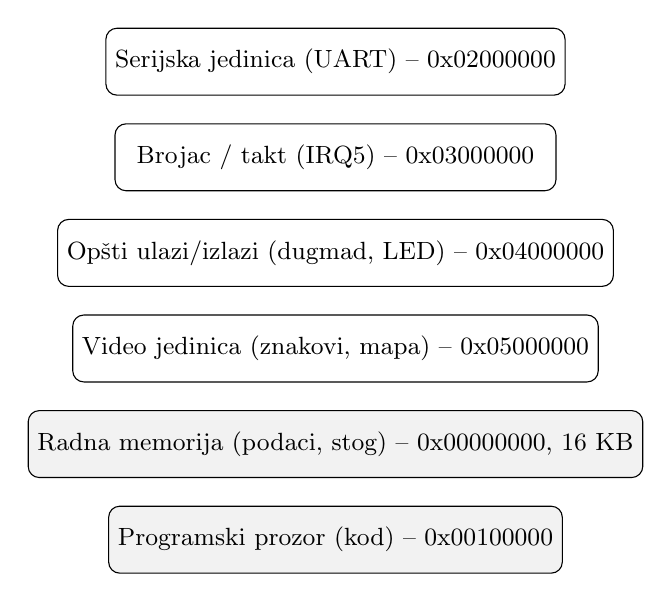
\begin{tikzpicture}[
    blok/.style={draw, rounded corners, minimum width=5.6cm, minimum height=0.85cm, align=center, font=\small},
    node distance=0.35cm
]
\node[blok] (uart) {Serijska jedinica (UART) -- 0x02000000};
\node[blok, below=of uart] (timer) {Brojac / takt (IRQ5) -- 0x03000000};
\node[blok, below=of timer] (gpio) {Op\v{s}ti ulazi/izlazi (dugmad, LED) -- 0x04000000};
\node[blok, below=of gpio] (video) {Video jedinica (znakovi, mapa) -- 0x05000000};
\node[blok, below=of video, fill=black!5] (ram) {Radna memorija (podaci, stog) -- 0x00000000, 16 KB};
\node[blok, below=of ram, fill=black!5] (rom) {Programski prozor (kod) -- 0x00100000};
\end{tikzpicture}
\caption{Pojednostavljena adresna i memorijska organizacija sistema na \v{c}ipu.}
\label{fig:memorija}
\end{figure}

Razdvajanje programa i podataka, kao i veli\v{c}ine pojedinih memorija, kasnije
postaje sredi\v{s}nji problem pri uklapanju cijele igre sa video izlazom, jer
svaka od tih memorija tro\v{s}i ograni\v{c}enu blokovsku memoriju plo\v{c}e.

\section{Dokaz pokretanja na hardveru}
\label{sec:platforma-boot}

Prije bilo kakvog portanja aplikacije, potvrdjeno je da operativni sistem uop\v{s}te
radi na plo\v{c}i. Sintetizovan je sklop sa serijskim izlazom, a u njega je
ugra\dj{}en jednostavan program sa tri zadatka. Nakon upisa sklopa u memoriju
plo\v{c}e, preko serijske veze na brzini od sto petnaest hiljada bita u sekundi
dobijeni su o\v{c}ekivani ispisi zadataka i njihovo smjenjivanje. Time je
pokazano da takt raspore\dj{}iva\v{c}a, programski prekid za zamjenu konteksta i
me\dj{}usobno isklju\v{c}ivanje pristupa serijskoj jedinici rade ispravno.

\section{Zaklju\v{c}ak poglavlja}
\label{sec:platforma-zakljucak}

U poglavlju je predstavljena hardverska osnova rada. Opisani su plo\v{c}a Tang
Nano 9K i meki procesor PicoRV32, prilago\dj{}eni port operativnog sistema
FreeRTOS sa taktom iz vanjskog brojaca i zamjenom konteksta putem programskog
prekida, te organizacija memorije i perifernih jedinica. Potvr\dj{}eno je da
sistem radi na stvarnom hardveru. Ova osnova omogu\'cava da se u narednom
poglavlju pristupi razdvajanju aplikacije na zasebne zadatke.

% ============================================================================
\chapter{Razdvajanje aplikacije na zadatke}
\label{ch:zadaci}
% ============================================================================

U ovom poglavlju opisuje se kako je monolitna aplikacija TetriSaraj prevedena u
skup zasebnih zadataka pod upravom raspore\dj{}iva\v{c}a. Najprije se obja\v{s}njava
razdvajanje \v{c}iste logike igre od dijela koji pristupa hardveru, jer je takvo
razdvajanje preduslov za rad pod operativnim sistemom. Zatim se opisuje
arhitektura zadataka i na\v{c}ini njihove komunikacije. Na kraju se prikazuje
dokaz da logika igre zaista napreduje pod raspore\dj{}iva\v{c}em na stvarnom
hardveru, i to bez video izlaza, kako bi se prvo potvrdila ispravnost samog
toka igre. Ovaj korak je va\v{z}an jer odvaja pitanje ispravnosti logike od
kasnijeg pitanja uklapanja video izlaza.

\section{Razdvajanje logike igre i pristupa hardveru}
\label{sec:zadaci-razdvajanje}

Izvorna aplikacija dr\v{z}ala je stanje igre u globalnim promjenljivim i
direktno pristupala perifernim jedinicama unutar jedne velike petlje. Da bi se
igra mogla izvr\v{s}avati kao zadatak, kod je razdvojen na dva dijela. Prvi dio
\v{c}ini \v{c}ista logika igre koja radi isklju\v{c}ivo nad strukturom stanja u
memoriji, bez ikakvog pristupa hardveru. Drugi dio \v{c}ini sloj platforme koji
obavlja pristup serijskoj jedinici, dugmadima i video memoriji. Takvo
razdvajanje omogu\'cava da se ista logika igre koristi i u ina\v{c}ici sa video
izlazom i u ina\v{c}ici koja stanje ispisuje tekstualno preko serijske veze.

\section{Arhitektura zadataka i komunikacija}
\label{sec:zadaci-arhitektura}

Aplikacija je podijeljena na \v{c}etiri zadatka razli\v{c}itih prioriteta.
Zadatak za unos periodi\v{c}no o\v{c}itava ulaz i \v{s}alje ga dalje. Zadatak
igre prima posljednji unos i pomjera stanje igre naprijed na zadatom periodu.
Zadatak za iscrtavanje osvje\v{z}ava prikaz kada se stanje promijeni. Pomo\'cni
zadatak periodi\v{c}no ispisuje stanje sistema preko serijske veze. Za prenos
unosa koristi se red poruka, a za za\v{s}titu zajedni\v{c}kog stanja igre koristi
se me\dj{}usobno isklju\v{c}ivanje. Ova organizacija prikazana je na slici
\ref{fig:zadaci}.

\begin{figure}[H]
\centering
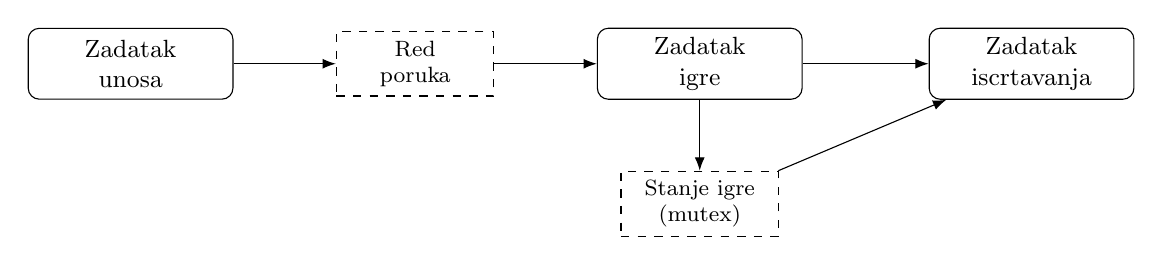
\begin{tikzpicture}[
    taskbox/.style={draw, rounded corners, minimum width=2.6cm, minimum height=0.9cm, align=center, font=\small},
    combox/.style={draw, dashed, minimum width=2.0cm, minimum height=0.8cm, align=center, font=\footnotesize},
    >=Latex
]
\node[taskbox] (unos) {Zadatak\\ unosa};
\node[combox, right=1.3cm of unos] (red) {Red\\ poruka};
\node[taskbox, right=1.3cm of red] (igra) {Zadatak\\ igre};
\node[taskbox, right=1.6cm of igra] (render) {Zadatak\\ iscrtavanja};
\node[combox, below=0.9cm of igra] (mutex) {Stanje igre\\ (mutex)};

\draw[->] (unos) -- (red);
\draw[->] (red) -- (igra);
\draw[->] (igra) -- (render);
\draw[->] (igra) -- (mutex);
\draw[->] (mutex) -- (render);
\end{tikzpicture}
\caption{Arhitektura zadataka: unos se prenosi redom poruka, a zajedni\v{c}ko stanje igre \v{s}titi se me\dj{}usobnim isklju\v{c}ivanjem.}
\label{fig:zadaci}
\end{figure}

Razdvajanje na zadatke razli\v{c}itih prioriteta omogu\'cava da zadatak igre ima
prednost nad iscrtavanjem, a da unos ima najve\'cu prednost. Time se postavlja
osnova za predvidljivo pona\v{s}anje sistema u realnom vremenu.

\section{Dokaz rada na hardveru bez video izlaza}
\label{sec:zadaci-headless}

Da bi se ispravnost logike potvrdila prije slo\v{z}enog uklapanja video izlaza,
napravljena je ina\v{c}ica koja stanje igre iscrtava tekstualno preko serijske
veze, bez pristupa video memoriji. Takva ina\v{c}ica uklapa se u ve\'c provjereni
sklop sa serijskim izlazom. Nakon upisa u plo\v{c}u, preko serijske veze
dobijeni su okviri stanja igre. U njima se vidi okvir polja, padaju\'ca figura,
te promjena rezultata kada se figura zaklju\v{c}a i pojavi nova. Skra\'ceni
ispis prikazan je u listingu \ref{lst:headless}.

\begin{lstlisting}[caption={Skra\'ceni serijski ispis tekstualne ina\v{c}ice: rezultat raste sa 0x0000 na 0x0001 nakon zaklju\v{c}avanja figure.}, label={lst:headless}]
--- frame 0x0002  score=0x0000  lives=0x03
########################################
            IIII   ##
########################################
[hb] beat=0x0002 tick=0x0000019C score=0x0000 ...

--- frame 0x0003  score=0x0001  lives=0x03
 OOO               ##
  O                ##
########################################
\end{lstlisting}

Ispis pokazuje da takt raspore\dj{}iva\v{c}a napreduje, da \v{c}etiri zadatka
sara\dj{}uju preko reda poruka i me\dj{}usobnog isklju\v{c}ivanja bez naru\v{s}avanja
ispisa, te da stvarna logika igre napreduje kroz pojavu, padanje, zaklju\v{c}avanje
i bodovanje figura. Time je dokazano da je igra pod upravom operativnog sistema
funkcionalna na hardveru.

\section{Zaklju\v{c}ak poglavlja}
\label{sec:zadaci-zakljucak}

U poglavlju je prikazano razdvajanje aplikacije na \v{c}istu logiku i sloj
platforme, te podjela na \v{c}etiri zadatka koji komuniciraju redom poruka i
me\dj{}usobnim isklju\v{c}ivanjem. Rad logike igre pod raspore\dj{}iva\v{c}em
potvr\dj{}en je na hardveru putem tekstualnog ispisa, \v{c}ime je ispravnost toka
igre odvojena od pitanja video izlaza. Time su stvoreni uslovi da se u narednom
poglavlju rije\v{s}i uklapanje cijele igre zajedno sa video izlazom.

% ============================================================================
\chapter{Uklapanje cijele igre sa video izlazom}
\label{ch:uklapanje}
% ============================================================================

U ovom poglavlju obra\dj{}uje se sredi\v{s}nji in\v{z}enjerski problem rada, a to
je uklapanje cijele igre zajedno sa operativnim sistemom i video izlazom u
stroge resurse plo\v{c}e Tang Nano 9K. Najprije se opisuje problem koji se javio
pri prvom poku\v{s}aju, zatim se analizira njegov stvarni uzrok kroz zauze\'ce
blokovske memorije. Nakon toga prikazuju se dva rje\v{s}enja koja su zajedno
omogu\'cila uklapanje, kao i jedno va\v{z}no otkri\'ce o pona\v{s}anju alata za
sintezu. Na kraju se daje kona\v{c}ni rezultat uklapanja i prilagodba video
inicijalizacije. Ovo poglavlje predstavlja te\v{z}i\v{s}te tehni\v{c}kog
doprinosa rada.

\section{Problem uklapanja}
\label{sec:uklapanje-problem}

Pri prvom poku\v{s}aju spajanja procesora sa operativnim sistemom i video
jedinicom u rezoluciji visoke definicije, sinteza nije uspjela. Procijenjeni
broj logi\v{c}kih elemenata iznosio je oko \v{s}esnaest hiljada, dok plo\v{c}a
raspola\v{z}e sa oko osam i po hiljada. Na prvi pogled \v{c}inilo se da je
problem u koli\v{c}ini logike, me\dj{}utim, dublja analiza pokazala je da je
stvarni uzrok bio drugdje.

\section{Analiza zauze\'ca blokovske memorije}
\label{sec:uklapanje-analiza}

Pregledom izvje\v{s}taja sinteze utvr\dj{}eno je da je ve\'c sama ina\v{c}ica sa
serijskim izlazom tro\v{s}ila svu raspolo\v{z}ivu blokovsku memoriju, odnosno
svih dvadeset \v{s}est blokova. Od toga je programska memorija zauzimala
\v{s}esnaest blokova, radna memorija osam, a serijska jedinica dva. Kako vi\v{s}e
nije bilo slobodne blokovske memorije, video jedinica je svoju znakovnu i mapnu
memoriju morala smjestiti u logi\v{c}ke elemente i registre, \v{s}to je dovelo do
prividne eksplozije broja logi\v{c}kih elemenata. Drugim rije\v{c}ima, problem
nije bio u logici, nego u nedostatku blokovske memorije.

Pri poku\v{s}aju smanjenja memorija uo\v{c}eno je i va\v{z}no svojstvo alata za
sintezu. Alat pouzdano prepoznaje i smje\v{s}ta memoriju u blokovsku memoriju
samo kada je njena dubina jednaka stepenu broja dva. Kada je programska memorija
poku\v{s}ana smanjiti na dubinu koja nije stepen broja dva, alat je memoriju
po\v{c}eo realizovati pomo\'cu registara, \v{s}to je dovelo do gotovo devetnaest
hiljada registara i nove neuspjele sinteze. Ovo otkri\'ce odredilo je smjer
svih daljih optimizacija, jer su sve dubine memorija morale ostati stepeni broja
dva.

\section{Dva rje\v{s}enja: manji program i manja video memorija}
\label{sec:uklapanje-rjesenja}

Prvo rje\v{s}enje odnosi se na programsku memoriju. Utvr\dj{}eno je da je program
povezivao i one funkcije operativnog sistema koje se uop\v{s}te ne koriste. Uz
prevo\dj{}enje sa razdvajanjem funkcija u zasebne sekcije i uklanjanjem
nekori\v{s}tenih sekcija pri povezivanju, veli\v{c}ina programa smanjena je sa
oko dvadeset dva i po hiljade bajta na oko petnaest hiljada bajta. Time je
program pao ispod granice od \v{s}esnaest kilobajta, pa programska memorija sada
zauzima osam umjesto \v{s}esnaest blokova.

Drugo rje\v{s}enje odnosi se na video memoriju. Umjesto rezolucije visoke
definicije, kori\v{s}tena je ni\v{z}a rezolucija, \v{c}ime se znakovna memorija
smanjila sa dvanaest hiljada dvije stotine osamdeset osam na \v{c}etiri hiljade
devedeset \v{s}est rije\v{c}i. Obje veli\v{c}ine ostale su stepeni broja dva,
\v{s}to je u skladu sa ranije opisanim svojstvom alata. Zajedno, ova dva
rje\v{s}enja oslobodila su dovoljno blokovske memorije da se cijeli sistem
uklopi.

\section{Rezultat uklapanja i prilagodba video inicijalizacije}
\label{sec:uklapanje-rezultat}

Nakon primjene oba rje\v{s}enja, sinteza je uspjela, a sistem se uklopio u
resurse plo\v{c}e sa odre\dj{}enom rezervom. Pore\dj{}enje zauze\'ca resursa prije
i poslije optimizacije dato je u tabeli \ref{table:resursi}.

\begin{table}[H]
\caption{Zauze\'ce resursa kombinovanog sistema prije i poslije optimizacije.}
\label{table:resursi}
\begin{center}
\begin{tabular}{lcc}
\hline
Resurs & Prije & Poslije \\ \hline
Logi\v{c}ki elementi & 16041 (prekora\v{c}eno) & 3348 / 8640 \\
Registri & -- & 1349 / 6693 \\
Blokovska memorija & 26 / 26 & 22 / 26 \\
\quad programska (pROM) & 16 & 8 \\
\quad radna (SP) & 8 & 8 \\
\quad ostalo (SDPB) & 2 & 6 \\ \hline
\end{tabular}
\end{center}
\end{table}

Nakon \v{s}to je sklop uklopljen, prilago\dj{}ena je i video inicijalizacija u
programu. Po\v{s}to je mapa polja ista u obje rezolucije, jer se polje sastoji od
istog broja velikih znakova, mijenjala se samo veli\v{c}ina pojedinog znaka.
Inicijalizacija znakova prilago\dj{}ena je da upisuje znakove veli\v{c}ine
\v{s}esnaest sa \v{s}esnaest ta\v{c}aka umjesto ranijih dvadeset \v{c}etiri sa
trideset dvije. Sistem se nakon toga uspje\v{s}no pokre\'ce na hardveru i video
inicijalizacija se izvr\v{s}ava do kraja, dok kona\v{c}na vizuelna potvrda slike
na ekranu ostaje stavka za daljnji rad.

\section{Zaklju\v{c}ak poglavlja}
\label{sec:uklapanje-zakljucak}

U poglavlju je rije\v{s}en glavni in\v{z}enjerski problem rada. Pokazano je da
uzrok neuspjeha prvog uklapanja nije bila koli\v{c}ina logike, nego nedostatak
blokovske memorije, te da alat za sintezu pouzdano koristi blokovsku memoriju
samo za dubine koje su stepeni broja dva. Smanjenjem programa uklanjanjem
nekori\v{s}tenih funkcija i kori\v{s}tenjem ni\v{z}e video rezolucije sistem je
uklopljen u resurse plo\v{c}e i pokrenut na hardveru. Time je pokazano da je
cijela igra sa operativnim sistemom i video izlazom izvodljiva na ovoj
niskobud\v{z}etnoj plo\v{c}i.

% ============================================================================
\chapter{Mjerenje zamjene konteksta i pore\dj{}enje sa simulatorom}
\label{ch:mjerenje}
% ============================================================================

U ovom poglavlju opisuje se mjerenje vremena zamjene konteksta operativnog
sistema na stvarnom hardveru, te njegovo pore\dj{}enje sa ranije dobijenim
vrijednostima iz simulatora. Najprije se obja\v{s}njava metodologija mjerenja i
razlog za odre\dj{}ene odluke pri njenoj izradi. Zatim se prikazuju izmjereni
rezultati na hardveru. Na kraju se ti rezultati pa\v{z}ljivo pore\dj{}uju sa
rezultatima iz simulatora, uz jasno isticanje ograni\v{c}enja takvog pore\dj{}enja.
Cilj poglavlja je dati prvu mjerljivu karakterizaciju operativnog sistema na
ovoj platformi, bez preuveli\v{c}avanja zaklju\v{c}aka.

\section{Metodologija mjerenja}
\label{sec:mjerenje-metoda}

Mjerenje oponasa test zamjene konteksta iz simulatorskog dijela istra\v{z}ivanja
\citep{thesisqemu}. Jedna iteracija obuhvata dvije zamjene konteksta, odlazak iz
prvog u drugi zadatak i povratak nazad. Vrijeme se mjeri slobodnim hardverskim
broja\v{c}em koji radi na frekvenciji od dvadeset sedam megaherca. Za razliku od
simulatorskog testa, koji koristi dva zadatka istog prioriteta i jedan semafor,
\v{c}ije pona\v{s}anje zavisi od dijeljenja vremena, ovdje su kori\v{s}tena dva
semafora i zadatak odgovara\v{c} vi\v{s}eg prioriteta. Time svaka predaja semafora
sigurno izaziva mjerenu zamjenu konteksta. Mjerena veli\v{c}ina je ista, broj
takta za dvostruku zamjenu konteksta, a jednostruka zamjena dobija se dijeljenjem
sa dva.

\section{Rezultati na hardveru}
\label{sec:mjerenje-rezultati}

Mjereno je pet stotina iteracija, a rezultat je bio ponovljiv kroz vi\v{s}e
upisa u plo\v{c}u. Dobijene vrijednosti za dvostruku zamjenu konteksta iznose
sedam hiljada \v{s}ezdeset jedan takt kao najmanja, sedam hiljada sedamdeset
devet kao prosje\v{c}na i sedam hiljada devet stotina osamdeset dva kao najve\'ca
vrijednost. To odgovara prosje\v{c}nom vremenu od oko dvije stotine \v{s}ezdeset
dvije mikrosekunde. Jednostruka zamjena konteksta iznosi oko tri hiljade pet
stotina trideset takta, odnosno oko sto trideset jednu mikrosekundu. Mali raspon
izme\dj{}u najmanje i najve\'ce vrijednosti pokazuje da nijedan takt
raspore\dj{}iva\v{c}a nije upao u prozor mjerenja, pa su vrijednosti \v{c}iste.

Visok broj takta po zamjeni konteksta posljedica je toga \v{s}to je PicoRV32
vi\v{s}eciklusna jezgra na relativno niskoj frekvenciji, kako je opisano u
poglavlju \ref{ch:platforma}. Zamjena konteksta pohranjuje i obnavlja cijeli
skup cjelobrojnih registara, uz dodatni tro\v{s}ak rada sa semaforima.

\section{Pore\dj{}enje sa simulatorom}
\label{sec:mjerenje-poredjenje}

Rezultati iz simulatora, dobijeni emulacijom RISC-V sistema, daju za dvostruku
zamjenu konteksta najmanju vrijednost od devet hiljada sto osamdeset osam takta,
prosje\v{c}nu od dvadeset tri hiljade sedam stotina \v{c}etrdeset sedam i
najve\'cu od gotovo \v{c}etiri miliona takta. Pore\dj{}enje je dato u tabeli
\ref{table:poredjenje}.

\begin{table}[H]
\caption{Pore\dj{}enje dvostruke zamjene konteksta na hardveru i u simulatoru (u taktovima).}
\label{table:poredjenje}
\begin{center}
\begin{tabular}{lcc}
\hline
Veli\v{c}ina & Hardver (27 MHz) & Simulator (25 MHz) \\ \hline
Najmanja & 7061 & 9188 \\
Prosje\v{c}na & 7079 & 23747 \\
Najve\'ca & 7982 & 3895040 \\ \hline
\end{tabular}
\end{center}
\end{table}

Pore\dj{}enje treba tuma\v{c}iti oprezno. Hardverska vrijednost dobijena je
stvarnim broja\v{c}em takta, dok simulatorska vrijednost dolazi iz emuliranog
broja\v{c}a koji nije takovno ta\v{c}an u odnosu na stvarni \v{c}ip. Zbog toga se
ne pore\dj{}uju dva ista takta, nego model iz simulatora i stvarni hardver.
Najpo\v{s}tenija ta\v{c}ka pore\dj{}enja je najmanja vrijednost, jer nije optere\'cena
smetnjama, i tu su vrijednosti istog reda veli\v{c}ine. Prosje\v{c}na i najve\'ca
vrijednost u simulatoru znatno su ve\'ce zbog ka\v{s}njenja koja unosi
periodi\v{c}no \v{c}ekanje u testu i takt raspore\dj{}iva\v{c}a. Zbog svega
navedenog, ne iznosi se tvrdnja o ta\v{c}nom odnosu brzina, nego se zaklju\v{c}uje
da je izmjerena hardverska zamjena konteksta po redu veli\v{c}ine u skladu sa
\v{c}istom procjenom iz simulatora.

\section{Zaklju\v{c}ak poglavlja}
\label{sec:mjerenje-zakljucak}

U poglavlju je dato prvo mjerenje vremena zamjene konteksta operativnog sistema
na stvarnom hardveru. Opisana je metodologija, prikazani su ponovljivi rezultati
i izvr\v{s}eno je oprezno pore\dj{}enje sa simulatorom. Pokazano je da su \v{c}iste
vrijednosti istog reda veli\v{c}ine, ali i da razlike u izvoru takta i uslovima
mjerenja ne dopu\v{s}taju izvo\dj{}enje ta\v{c}nog odnosa brzina. Time je
zaokru\v{z}ena mjerljiva karakterizacija sistema na ovoj platformi.

% ============================================================================
\chapter{Pravci daljnjeg istra\v{z}ivanja}
\label{ch:pravci}
% ============================================================================

U ovom poglavlju izdvajaju se mogu\'ci pravci daljnjeg istra\v{z}ivanja koji
prirodno proizlaze iz ura\dj{}enog rada. Svaki pravac povezan je sa konkretnom
prazninom uo\v{c}enom u radu ili u pregledu literature iz poglavlja
\ref{ch:srodni}. Pravci su pore\dj{}ani od onih koji najvi\v{s}e doprinose
nau\v{c}noj vrijednosti rada prema onima koji predstavljaju \v{s}ire pro\v{s}irenje.
Cilj poglavlja je pokazati da postoje\'ci rezultati \v{c}ine osnovu za vi\v{s}e
zaokru\v{z}enih istra\v{z}iva\v{c}kih cjelina.

\section{Kvantifikacija tro\v{s}ka operativnog sistema}
\label{sec:pravci-overhead}

Najva\v{z}niji pravec jeste mjerenje tro\v{s}ka koji unosi operativni sistem u
odnosu na golo izvr\v{s}avanje. Ista operacija bi se izmjerila sa raspore\dj{}iva\v{c}em
i bez njega, \v{c}ime bi se dobila stvarna cijena upotrebe operativnog sistema na
ovoj mekoj jezgri. Ovaj pravec direktno odgovara na pitanje cijene koje je
\v{c}esto u sredi\v{s}tu literature o operativnim sistemima za rad u realnom
vremenu \citep{ulsolutions2022rtos}.

\section{Uskla\dj{}ivanje metrike i statisti\v{c}ka obrada}
\label{sec:pravci-metrika}

Mjerenje iz poglavlja \ref{ch:mjerenje} obuhvata i tro\v{s}ak rada sa semaforima.
Da bi se rezultat mogao pore\dj{}ivati sa literaturom, potrebno je dodatno
izmjeriti u\v{z}u, \v{c}istu zamjenu konteksta bez tog tro\v{s}ka. Uz to, umjesto
najmanje, prosje\v{c}ne i najve\'ce vrijednosti, rezultate bi trebalo izraziti
srednjom vrijedno\v{s}\'cu sa standardnom devijacijom i raspodjelom, te
karakterizovati podrhtavanje. Time bi mjerenja dobila statisti\v{c}ku strogost
koju nau\v{c}ni rad zahtijeva.

\section{Uticaj mikroarhitekture i skupa instrukcija}
\label{sec:pravci-mikroarhitektura}

Meka jezgra dopu\v{s}ta promjenu konfiguracije, na primjer uklju\v{c}ivanje
sa\v{z}etog skupa instrukcija ili sklopa za pomjeranje. Mjerenjem zamjene
konteksta pri razli\v{c}itim konfiguracijama dobili bi se trendovi koji povezuju
mikroarhitekturu sa cijenom operativnog sistema. Ovaj pravec je u skladu sa
istra\v{z}ivanjima koja zajedno posmatraju mikroarhitekturu i operativni sistem
\citep{scheck2026coexploration}.

\section{Latencija i determinizam prekida pod optere\'cenjem}
\label{sec:pravci-prekidi}

Pored zamjene konteksta, va\v{z}na veli\v{c}ina je latencija prekida i njena
postojanost pod razli\v{c}itim optere\'cenjem sistema. Mjerenjem latencije
prekida i podrhtavanja, uz vi\v{s}e zadataka i ve\'ce optere\'cenje, ocijenila bi
se predvidljivost sistema, \v{s}to je klju\v{c}no svojstvo sistema za rad u
realnom vremenu.

\section{Sistematsko pore\dj{}enje simulatora i hardvera}
\label{sec:pravci-qemu}

Po\v{s}to je emulator QEMU funkcijski ta\v{c}an, a ne takovno ta\v{c}an
\citep{qemu}, zanimljivo je sistematski ispitati koliko dobro on predvi\dj{}a
vremenske veli\v{c}ine na stvarnom hardveru. Pore\dj{}enjem vi\v{s}e mjera na obje
platforme dobio bi se sud o tome u kojim slu\v{c}ajevima je simulacija dovoljno
vjerodostojna, a u kojima nije.

\section{Hardversko ubrzanje raspore\dj{}ivanja}
\label{sec:pravci-hardver}

Kona\v{c}no, budu\'ci da je rije\v{c} o mekoj jezgri na programabilnoj logici,
otvara se mogu\'cnost dodavanja namjenskog sklopa za ubrzanje raspore\dj{}ivanja
ili zamjene konteksta. Takav pristup je u literaturi pokazao zna\v{c}ajna
ubrzanja \citep{balas2023cv32rt}, a ovaj rad pru\v{z}a polaznu osnovu i mjerni
okvir naspram kojeg bi se takvo ubrzanje moglo vrednovati.

\section{Zaklju\v{c}ak poglavlja}
\label{sec:pravci-zakljucak}

U poglavlju je izlo\v{z}eno \v{s}est pravaca daljnjeg istra\v{z}ivanja, od
kvantifikacije tro\v{s}ka operativnog sistema i statisti\v{c}ke obrade mjerenja,
preko uticaja mikroarhitekture i pona\v{s}anja prekida, do sistematskog
pore\dj{}enja sa simulatorom i hardverskog ubrzanja raspore\dj{}ivanja. Svaki
pravec se naslanja na postoje\'ce rezultate i prazninu u literaturi, \v{c}ime se
pokazuje da rad ima jasan potencijal za nastavak.

% ---- Opci zakljucak (ne numerise se) ---------------------------------------
\chapter*{Zaklju\v{c}ak}
\addcontentsline{toc}{chapter}{Zaklju\v{c}ak}

U radu je prikazano portanje aplikacije TetriSaraj sa golog izvr\v{s}avanja na
operativni sistem za rad u realnom vremenu FreeRTOS, na otvorenoj RISC-V
platformi realizovanoj kao meki procesor PicoRV32 na plo\v{c}i Tang Nano 9K. Na
osnovu izlo\v{z}enog mo\v{z}e se zaklju\v{c}iti da je sva tri pitanja postavljena
u uvodu mogu\'ce potvrdno rije\v{s}iti. Aplikacija je uspje\v{s}no razdvojena na
\v{c}iste zadatke pod upravom raspore\dj{}iva\v{c}a, a njen rad je dokazan na
stvarnom hardveru putem serijskog ispisa u kojem logika igre napreduje. Cijeli
sistem, zajedno sa video izlazom, uklopljen je u stroge resurse plo\v{c}e i
pokrenut na hardveru. Kona\v{c}no, izmjereno je vrijeme zamjene konteksta na
stvarnom hardveru i oprezno upore\dj{}eno sa rezultatima iz simulatora.

Posebno je istaknuto otkri\'ce da uzrok neuspjelog uklapanja nije bila
koli\v{c}ina logike, nego nedostatak blokovske memorije, kao i to da alat za
sintezu pouzdano koristi blokovsku memoriju samo za dubine koje su stepeni broja
dva. Ta dva uvida bila su klju\v{c}na za uspje\v{s}no uklapanje sistema. Tako\dj{}er
je pokazano da su \v{c}iste vrijednosti zamjene konteksta na hardveru i u
simulatoru istog reda veli\v{c}ine.

Iako rad obuhvata cijeli put od porta operativnog sistema do mjerenja na
hardveru, pojedina pitanja ostaju otvorena za daljnje istra\v{z}ivanje.
Vizuelna potvrda kona\v{c}ne slike igre na ekranu nije zatvorena u okviru ovog
rada. Potpuno interaktivno upravljanje ograni\v{c}eno je malim brojem fizi\v{c}kih
dugmadi na plo\v{c}i. Tako\dj{}er, mjerenja bi se mogla pro\v{s}iriti na tro\v{s}ak
samog takta raspore\dj{}iva\v{c}a i na pona\v{s}anje sistema pod ve\'cim
optere\'cenjem. Ovi pravci predstavljaju prirodan nastavak rada.


\cleardoublepage
\phantomsection
\addcontentsline{toc}{chapter}{Popis slika}
\listoffigures

\cleardoublepage
\phantomsection
\addcontentsline{toc}{chapter}{Literatura}
\bibliographystyle{unsrtnat}
\bibliography{Reference}

\end{document}
